\section{RX1 \& RX2}

The sheets RX1 and RX2 are identical. They each consist of two amplifiers connected in series, shown
in Figure~\ref{fig:rx-sch}. The first amplifier is a
\href{http://www.skyworksinc.com/uploads/documents/SKY65404_31_201512J.pdf}{SKY65404} LNA which
operates in the 4.9GHz-5.9GHz range, has a gain of 13dB, a NF of 1dB and a P1dB of -4dBm. It is
hooked up exactly as specified in the datasheet, with the addition of a ferrite bead filtering its
power supply.

\begin{figure}[h]
  \centering
  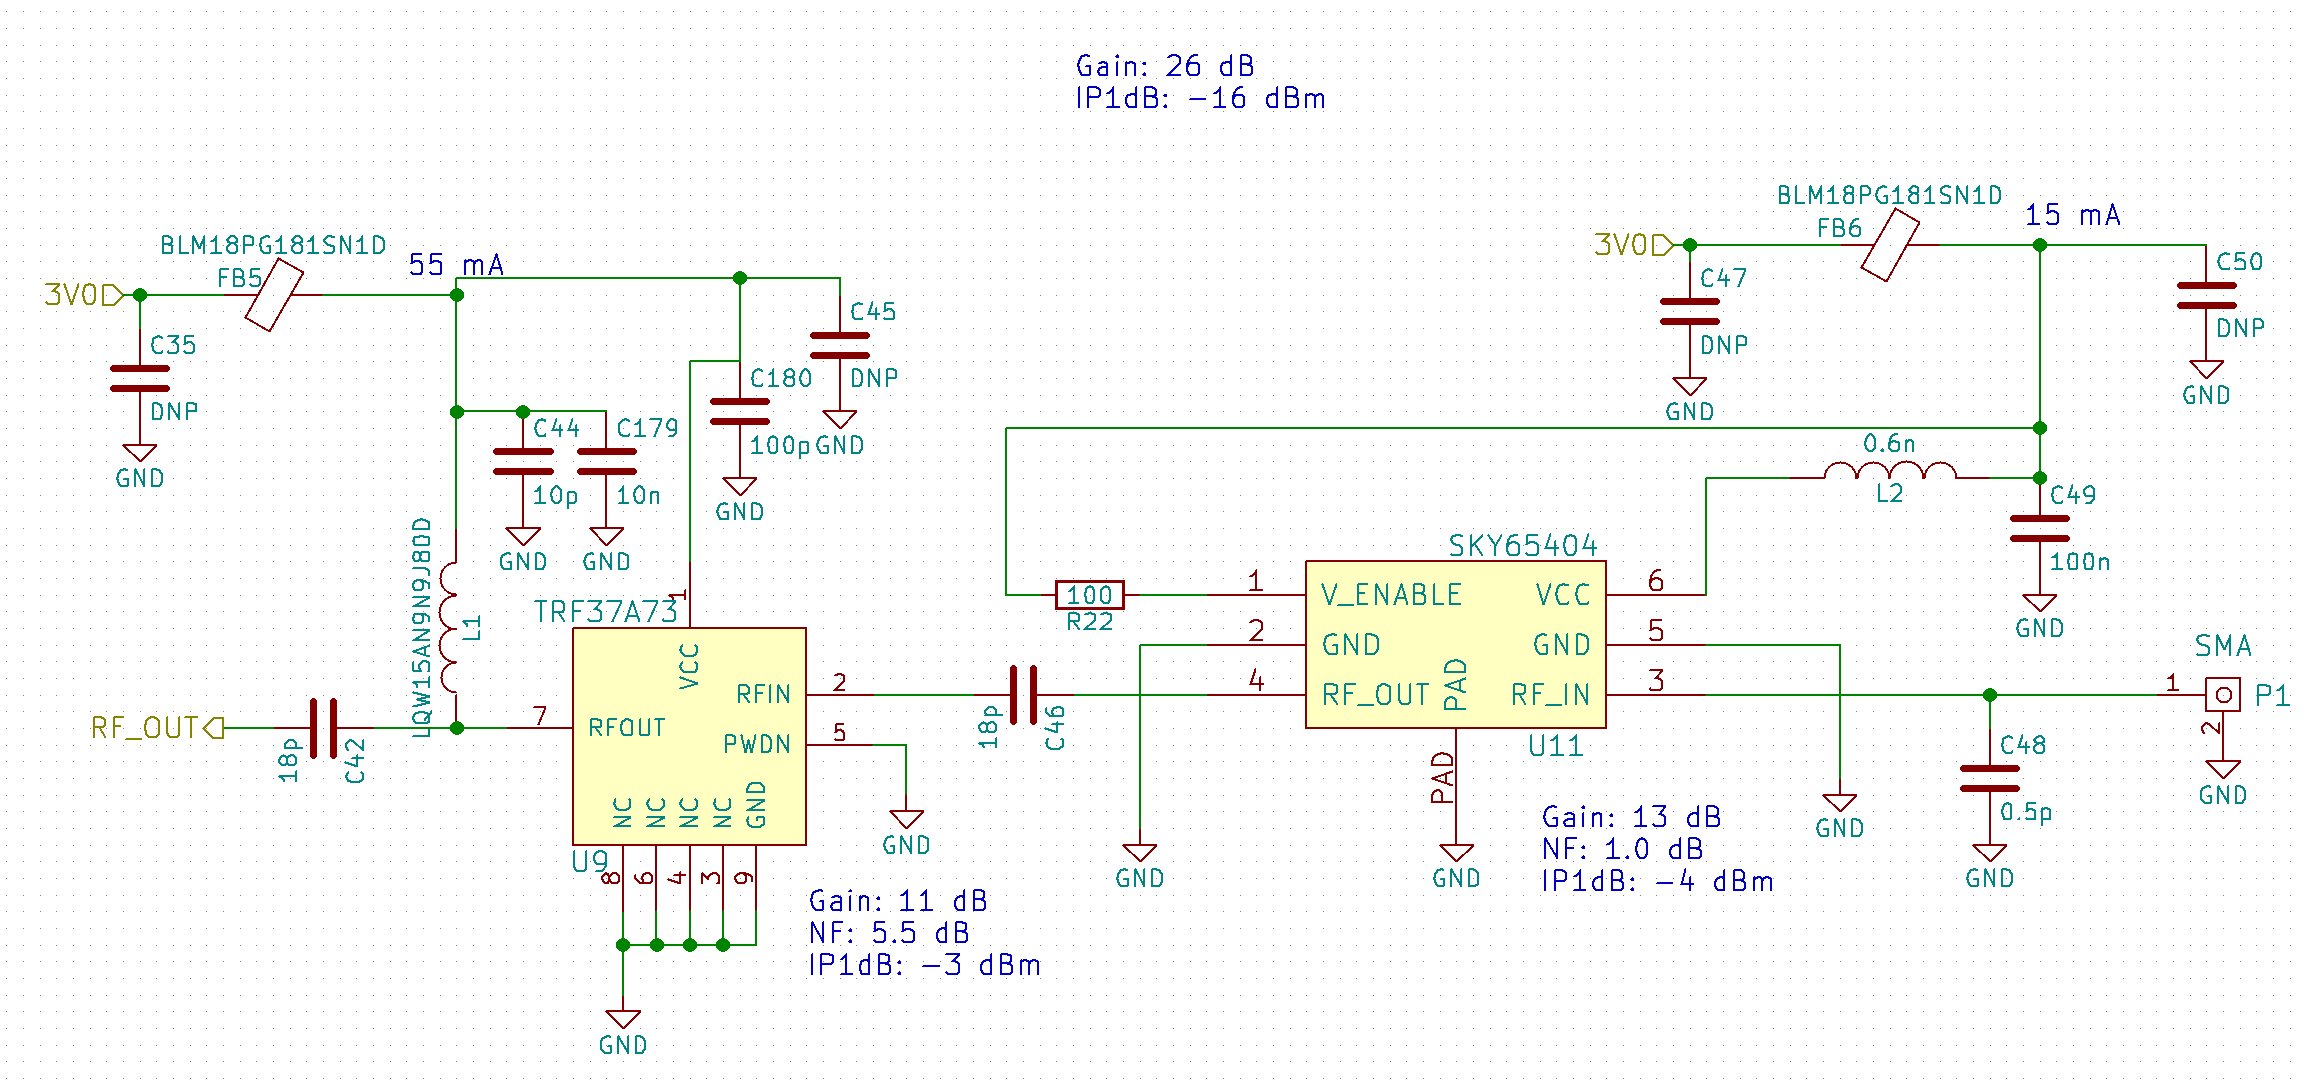
\includegraphics[width=\textwidth]{data/rx-sch.png}
  \caption{One of two RX schematic sheets. Both sheets are identical and consist of two amplifiers
    connected in series.}
  \label{fig:rx-sch}
\end{figure}

The second amplifier is a \href{http://www.ti.com/lit/ds/symlink/trf37a73.pdf}{TRF37A73} RF gain
amplifier. It is wired up as recommended in the datasheet, with the addition of a ferrite bead to
filter the power supply. Values for the various capacitors and inductor are left out of the
datasheet. A 100pF capacitor is used to short high frequency noise to the power supply, which is
typical of microwave devices. \textbf{\{START INCOMPLETE\}} I am not sure how the values for the RF
bypass capacitors, the inductor, and the DC blocking capacitors was chosen. Additionally, I'm not
sure how he arrives at a gain of 26dB, since I've read that gains in series should be additive (and
hence 24dB), and I'm not sure where the IP1dB value of -16dBm comes from \textbf{\{ENDINCOMPLETE\}}.